\documentclass{report} 
\setcounter{tocdepth}{0} 
\setcounter{secnumdepth}{4} 
\usepackage{lipsum,multicol,graphicx,float,subfig} 
\usepackage{hyperref}
\usepackage{titletoc} 
 
\begin{document} 
 
\title{\textbf{Vigneshwaran Radhakrishnan}} 
% \author{me} 
\date{\small Updated on \today} 
\maketitle 
 
%tell tex4ht to make main toc show only chapters 
%thanks to Radhakrishnan CV for this solution 
\ifdefined\HCode 
\Configure{tableofcontents*}{chapter} 
\fi 
 
% \tableofcontents 
 
\ifdefined\HCode 
\TocAt{chapter,section} %show section only in chapters TOC 
\TocAt{section,subsection} %show subsection only in sections TOC 
\fi 
 
%--------------------- 
\chapter{Home} 
\ifdefined\HCode 
\else 
{ 
\startcontents[chapter] 
\printcontents[chapter]{}{1}{\setcounter{tocdepth}{1}} 
} 
\fi 
      \section*{Vigneshwaran Radhakrishnan}

      % \begin{multicols}{2}
      %       \begin{itemize}
      %             \item Email: vigneshr@tamu.edu
      %             \item Phone: (979) 587-5208
      %             \item Office: HRBB 220
      %             \item \href{https://engineering.tamu.edu/aerospace/profiles/benzerga-amine.html}{Dr. Amine Benzerga}
      %             \item \href{Vignesh_CV.pdf}{Curriculum Vitae}
      %             \item \href{https://www.linkedin.com/in/vigneshwaranradhakrishnan/}{LinkedIn}
      %       \end{itemize}
      %       \columnbreak
            \begin{figure}[H]
                  \subfloat{
                        \begin{tabular}{l l}
                              Let &\\
                        \end{tabular}
                  }
                  \subfloat{
                        \centering
                        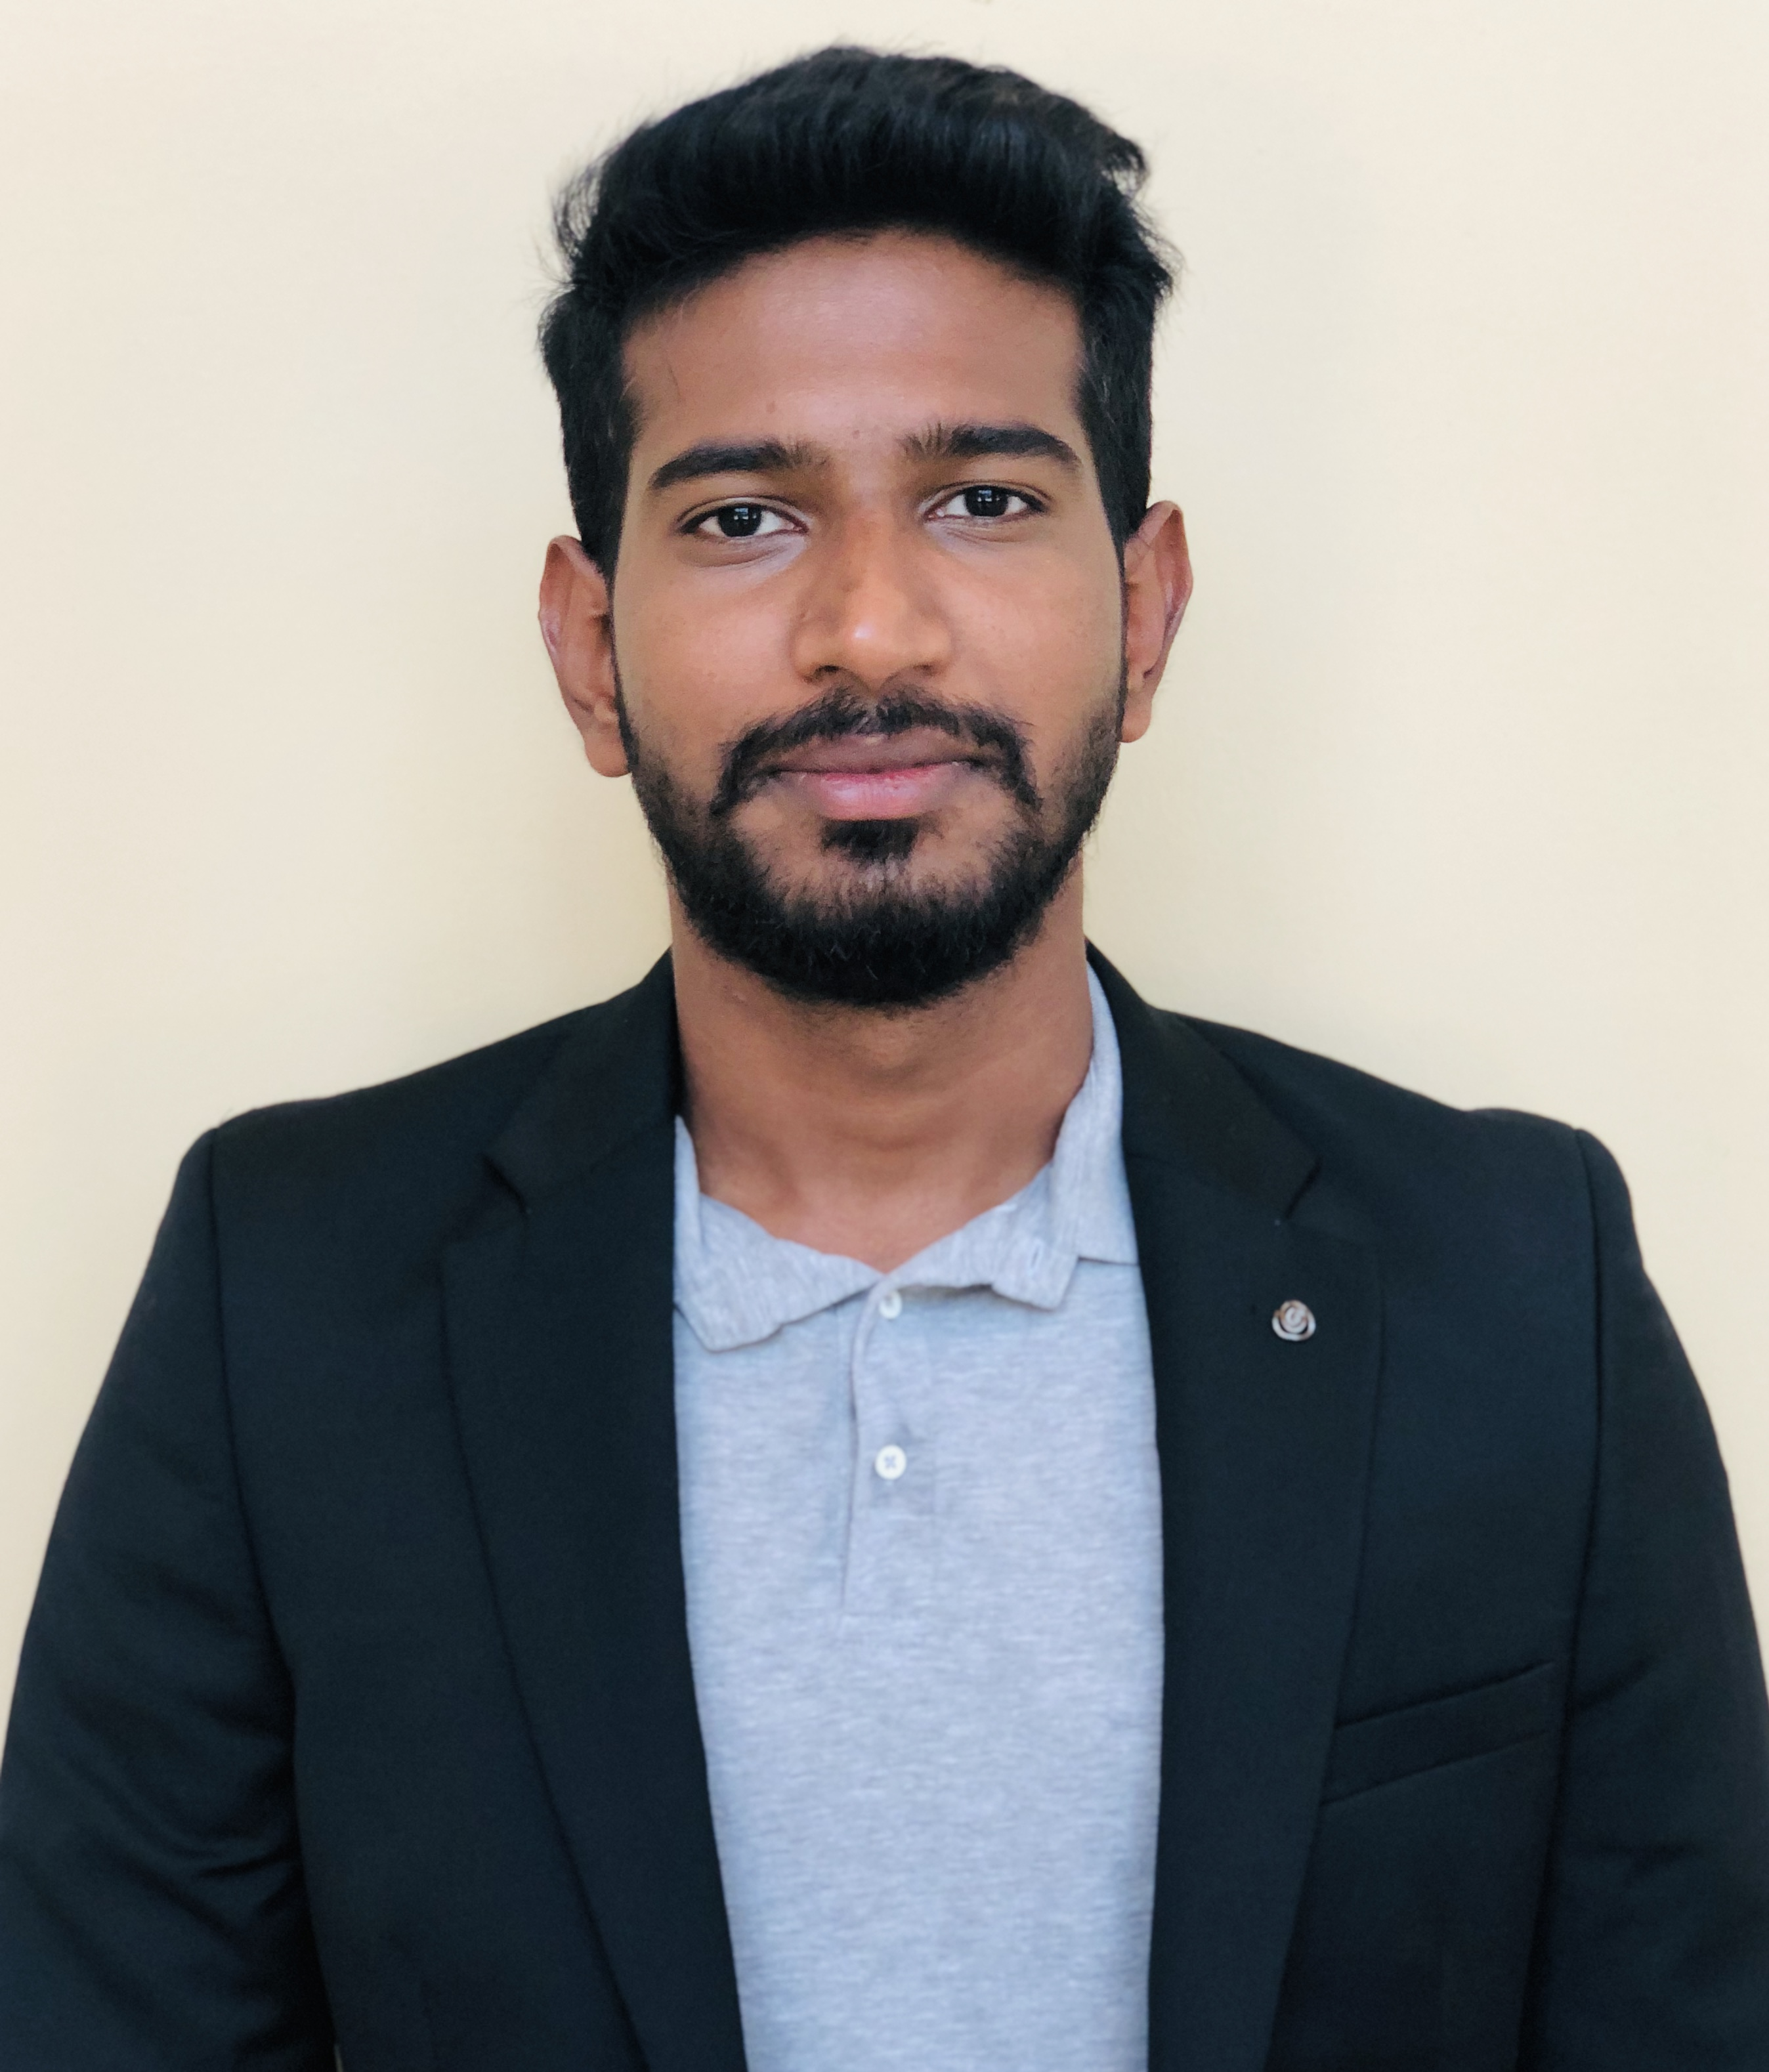
\includegraphics[width=0.3\textwidth]{Vignesh.eps}
                  }
            \end{figure}
      % \end{multicols}

      \section*{Biography}
 
  \section{section 1 in chapter 1} 
  \lipsum[1-2] 
 
  \section{section 2 in chapter 1} 
  \lipsum[1-2] 
  \subsection{subsection 1 in section 2 in chapter 1} 
  \lipsum[1-2] 
 
  \section{section 3 in chapter 1} 
  \lipsum[1-2] 
 
%--------------------- 
 
\ifdefined\HCode 
\PauseCutAt{section} 
\fi 
 
\ifdefined\HCode 
\else 
{ 
\stopcontents[chapter] 
} 
\fi 
 
 
\chapter{chapter 2} 
  \lipsum[10] 
 
  \section{section 1 in chapter 2} 
  \lipsum[1-2] 
 
  \section{section 2 in chapter 2} 
  \lipsum[1-2] 
  \subsection{subsection 1 in section 2 in chapter 2} 
  \lipsum[1-2] 
 
  \section{section 3 in chapter 2} 
  \lipsum[1-2] 
 
\end{document}